To understand whether LLMs can perform exploration, we consider perhaps the simplest RL problem, the \emph{multi-armed bandit} (MAB),
a well-studied setting that isolates the tradeoff between exploration (making decisions to gather information) and \emph{exploitation} (making the best decision given the available data).
Specifically, we consider a simple MAB problem with
$K$ possible actions, called \emph{arms}, indexed as $[K]:=\{1,\ldots,K\}$. Each arm $a$ is associated with mean reward $\mu_a\in[0,1]$, which is initially not known.
An agent interacts with the environment for $T$ time-steps, where in each time-step the agent selects an arm $a_t \in [K]$ and receives a reward $r_t$ drawn independently from a Bernoulli distribution with mean $\mu_{a_t}$.
The goal is to accumulate rewards, which roughly corresponds to identifying the arm whose distribution has the highest mean. Crucially, rewards for arms not chosen by the agent are
not revealed, so the agent must explore each arm to identify those
with high means.

\paragraph{Experiment setup}
For our main experiment, we consider an MAB instance with $K=5$ arms,
where the best arm has mean $\mu^\star = 0.6$, while the four sub-optimal arms each have mean $\mu = 0.4$. We set the time horizon to $T=100$. For baselines, we consider two standard MAB algorithms, \ucb and Thompson Sampling, which are known to be optimal in a certain theoretical/asymptotic sense. We also consider the \greedy algorithm, which does not explore and is known to fail.%
\footnote{In each round, \greedy chooses an arm with the largest average reward so far. The algorithm is initialized with one sample of each arm. It \emph{fails} in the sense that, with constant probability, it never chooses the best arm after initialization.}
While all three baselines have tunable parameters,
we perform no parameter tuning.  For baselines, we run $1000$ replicates (with the same mean rewards, but different realizations of the randomness).

We evaluate both \gptthree and \gptfour. To elicit the LLM to choose
one of the arms, we prompt the LLM with a description of the
decision-making problem and information about the history of
interaction thus far (see~\pref{fig:prompts}). Our prompt design allows two independent choices: the top sentence (\emph{framing}) and the way history is presented (\emph{raw} or \emph{summarized}). We always set the
temperature of the LLM to $0$, as this isolates ``deliberate''
exploration behavior of the model itself. For LLMs, we run $N=100$
replicates, where the only randomness is from the environment. Our basic prompt has the \emph{neutral} framing and \emph{raw} history. Intuitively, this prompt should make the problem more challenging for the LLM. However, such a prompt may better reflect real more-complex scenarios, where it is unclear how to summarize the history or provide a ``suggestive'' framing.


\begin{figure}
  \begin{center}
    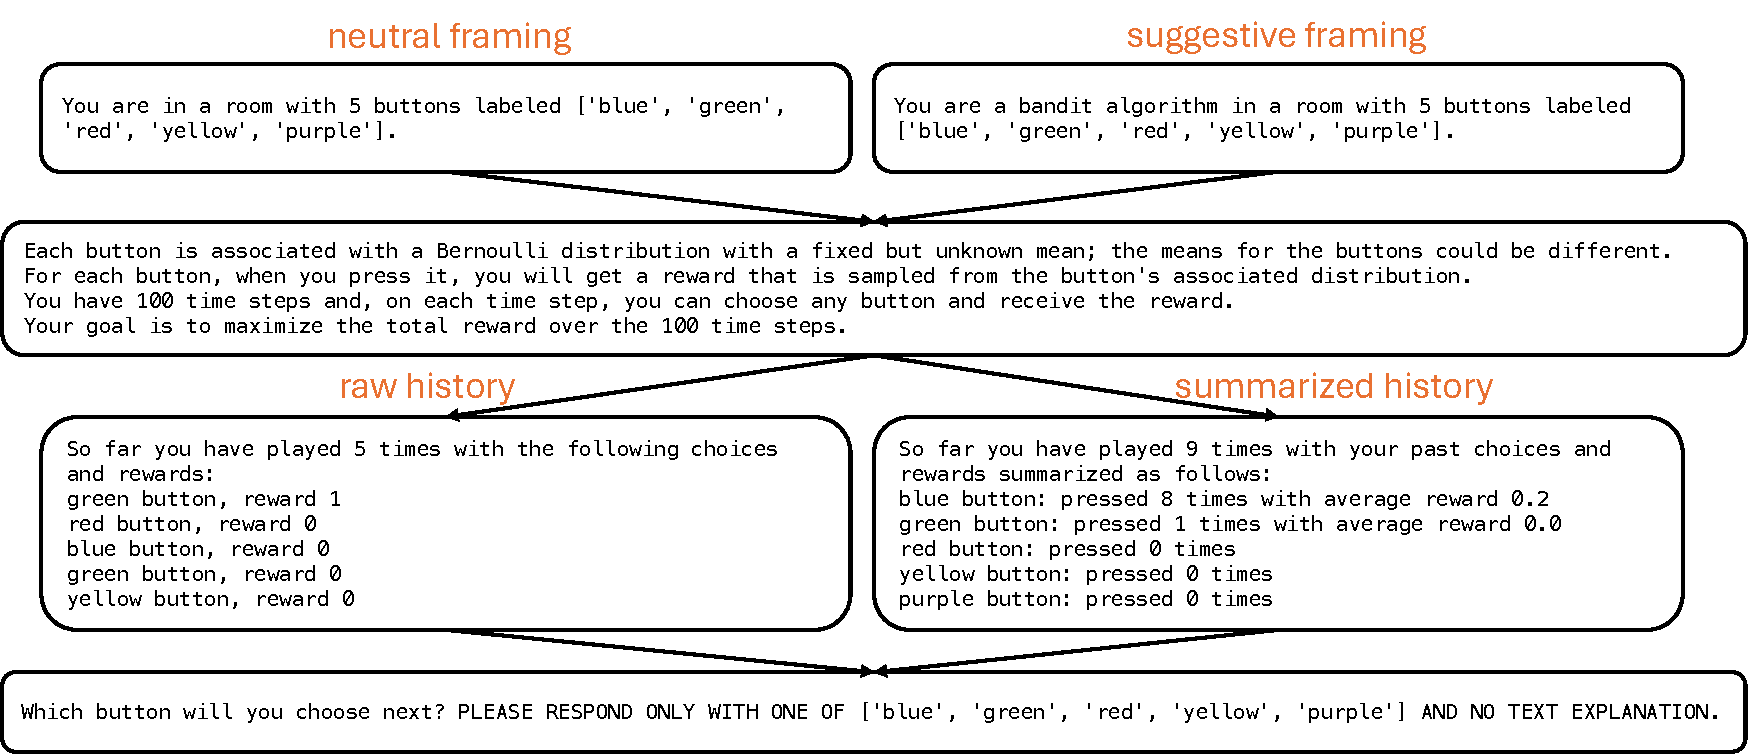
\includegraphics[width=\textwidth]{./prompt.pdf}
  \end{center}
  \vspace{-0.7cm}
  \caption{Prompts used in our experiments.}
  \vspace{-0.4cm}
  \label{fig:prompts}
\end{figure}

\subsection{Results}
Our main experiment uses the basic prompt, as discussed above.
The results are visualized in~\pref{fig:main}. We focus the discussion on \gptfour, since we find that \gptthree has quite poor performance in all of our experiments.


\gptfour exhibits \emph{highly bimodal} behavior,
whereby more than half of the $N=100$ replicates completely fail to
converge to the best arm and this is compensated by a few
replicates that converge extremely quickly. Indeed, here
we find that roughly $55\%$ of the replicates only choose the best
arm in fewer than $10/100$ time-steps, while roughly $10\%$ choose
the best arm almost every time (the left panel
of~\pref{fig:main}).

We also visualize a notion of \emph{persistent failure} of each
algorithm, measuring for each time-step $t$ the fraction of replicates
in which the LLM fails to select the best arm even once in the remaining
time-steps ${t,\ldots,T}$. Persistent failures are suggestive of a long-term
failure to explore which cannot be improved by running the algorithm
for longer. Consistent with the bimodal behavior, we also see that
\gptfour has a large fraction of persistent failures. These behaviors
are qualitatively similar to those of \greedy,
and qualitatively very different from those of \ucb and Thompson Sampling.

In terms total reward accumulated (averaged over replicates), \gptfour
slightly underperforms the baselines (the right panel
of~\pref{fig:main}). However, this summary conceals the failures
visualized in the previous two plots. Moreover, due to the persistent failures, we expect \gptfour to
perform much worse compared to the baselines when as the time horizon
($T$) and/or the problem complexity ($K$) increases.

As potential interventions to improve the performance of \gptfour, we
experiment with two other prompts: neutral framing with
summarized history and suggestive framing with summarized
history. These results are visualized in~\pref{fig:interventions}. We
find that the interventions help somewhat, but the undesirable
bimodal behavior remains.

We also performed several other experiments at a smaller scale as preliminary robustness checks and obtained qualitatively similar findings. These included experiments with other prompts and easier problem instances with larger gap $\mu^\star - \mu$ and/or  $K=2$ arms.
Due to limited access to \gptfour, we could not run these experiments at a larger scale, so we do not report the quantitative results here.



\begin{figure}[t]
  \begin{center}
    \includegraphics[width=\textwidth]{../figs/kbuttonssum_triple.pdf}\\
    \includegraphics[width=\textwidth]{../figs/kbanditssum_triple.pdf}
  \end{center}
  \vspace{-0.9cm}
  \caption{Top row: experimental results with a \emph{neutral} and \emph{summarized} prompt.  Bottom row:
    results with a \emph{suggestive} and \emph{summarized}
    prompt. Visualizations are the same as those
    in~\pref{fig:main}. Both interventions slightly improve
    performance for \gptfour, but bimodal behavior and persistent
    failures remain.}
\vspace{-0.4cm}
  \label{fig:interventions}
\end{figure}

